\documentclass[../../main.tex]{subfiles}

\begin{document}
\problem{13: What are the destination IP addresses for the two DNS queries? What do these IP addresses correspond to?}
\begin{wts}
What are the destination IP addresses for the two DNS queries? What do these IP addresses correspond to?
\end{wts}
\begin{proof}
It is clear that
\begin{quote}
    TCP is provides full-duplex data transport to the application layer by employing a sliding window mechanism. This requires both the sender and the receiver to maintain 1) the window size and 2) the expected sequence number of the other host, which advances (modulo $N$, where $N$ denotes the maximum sequence number) on the receipt of an acknowledgement.
\end{quote}
The first segment is sent from the client (the author’s computer) to the server, with the flag \code{SYN = 1}, and the client communicates to the server its
\begin{itemize}
    \item Window size $W_c$, the maximum number of bytes that the server should send without receiving an acknowledgement.
    \item Client initial sequence number, ${SEQ}_C$, a $32$-bit number 
\end{itemize}
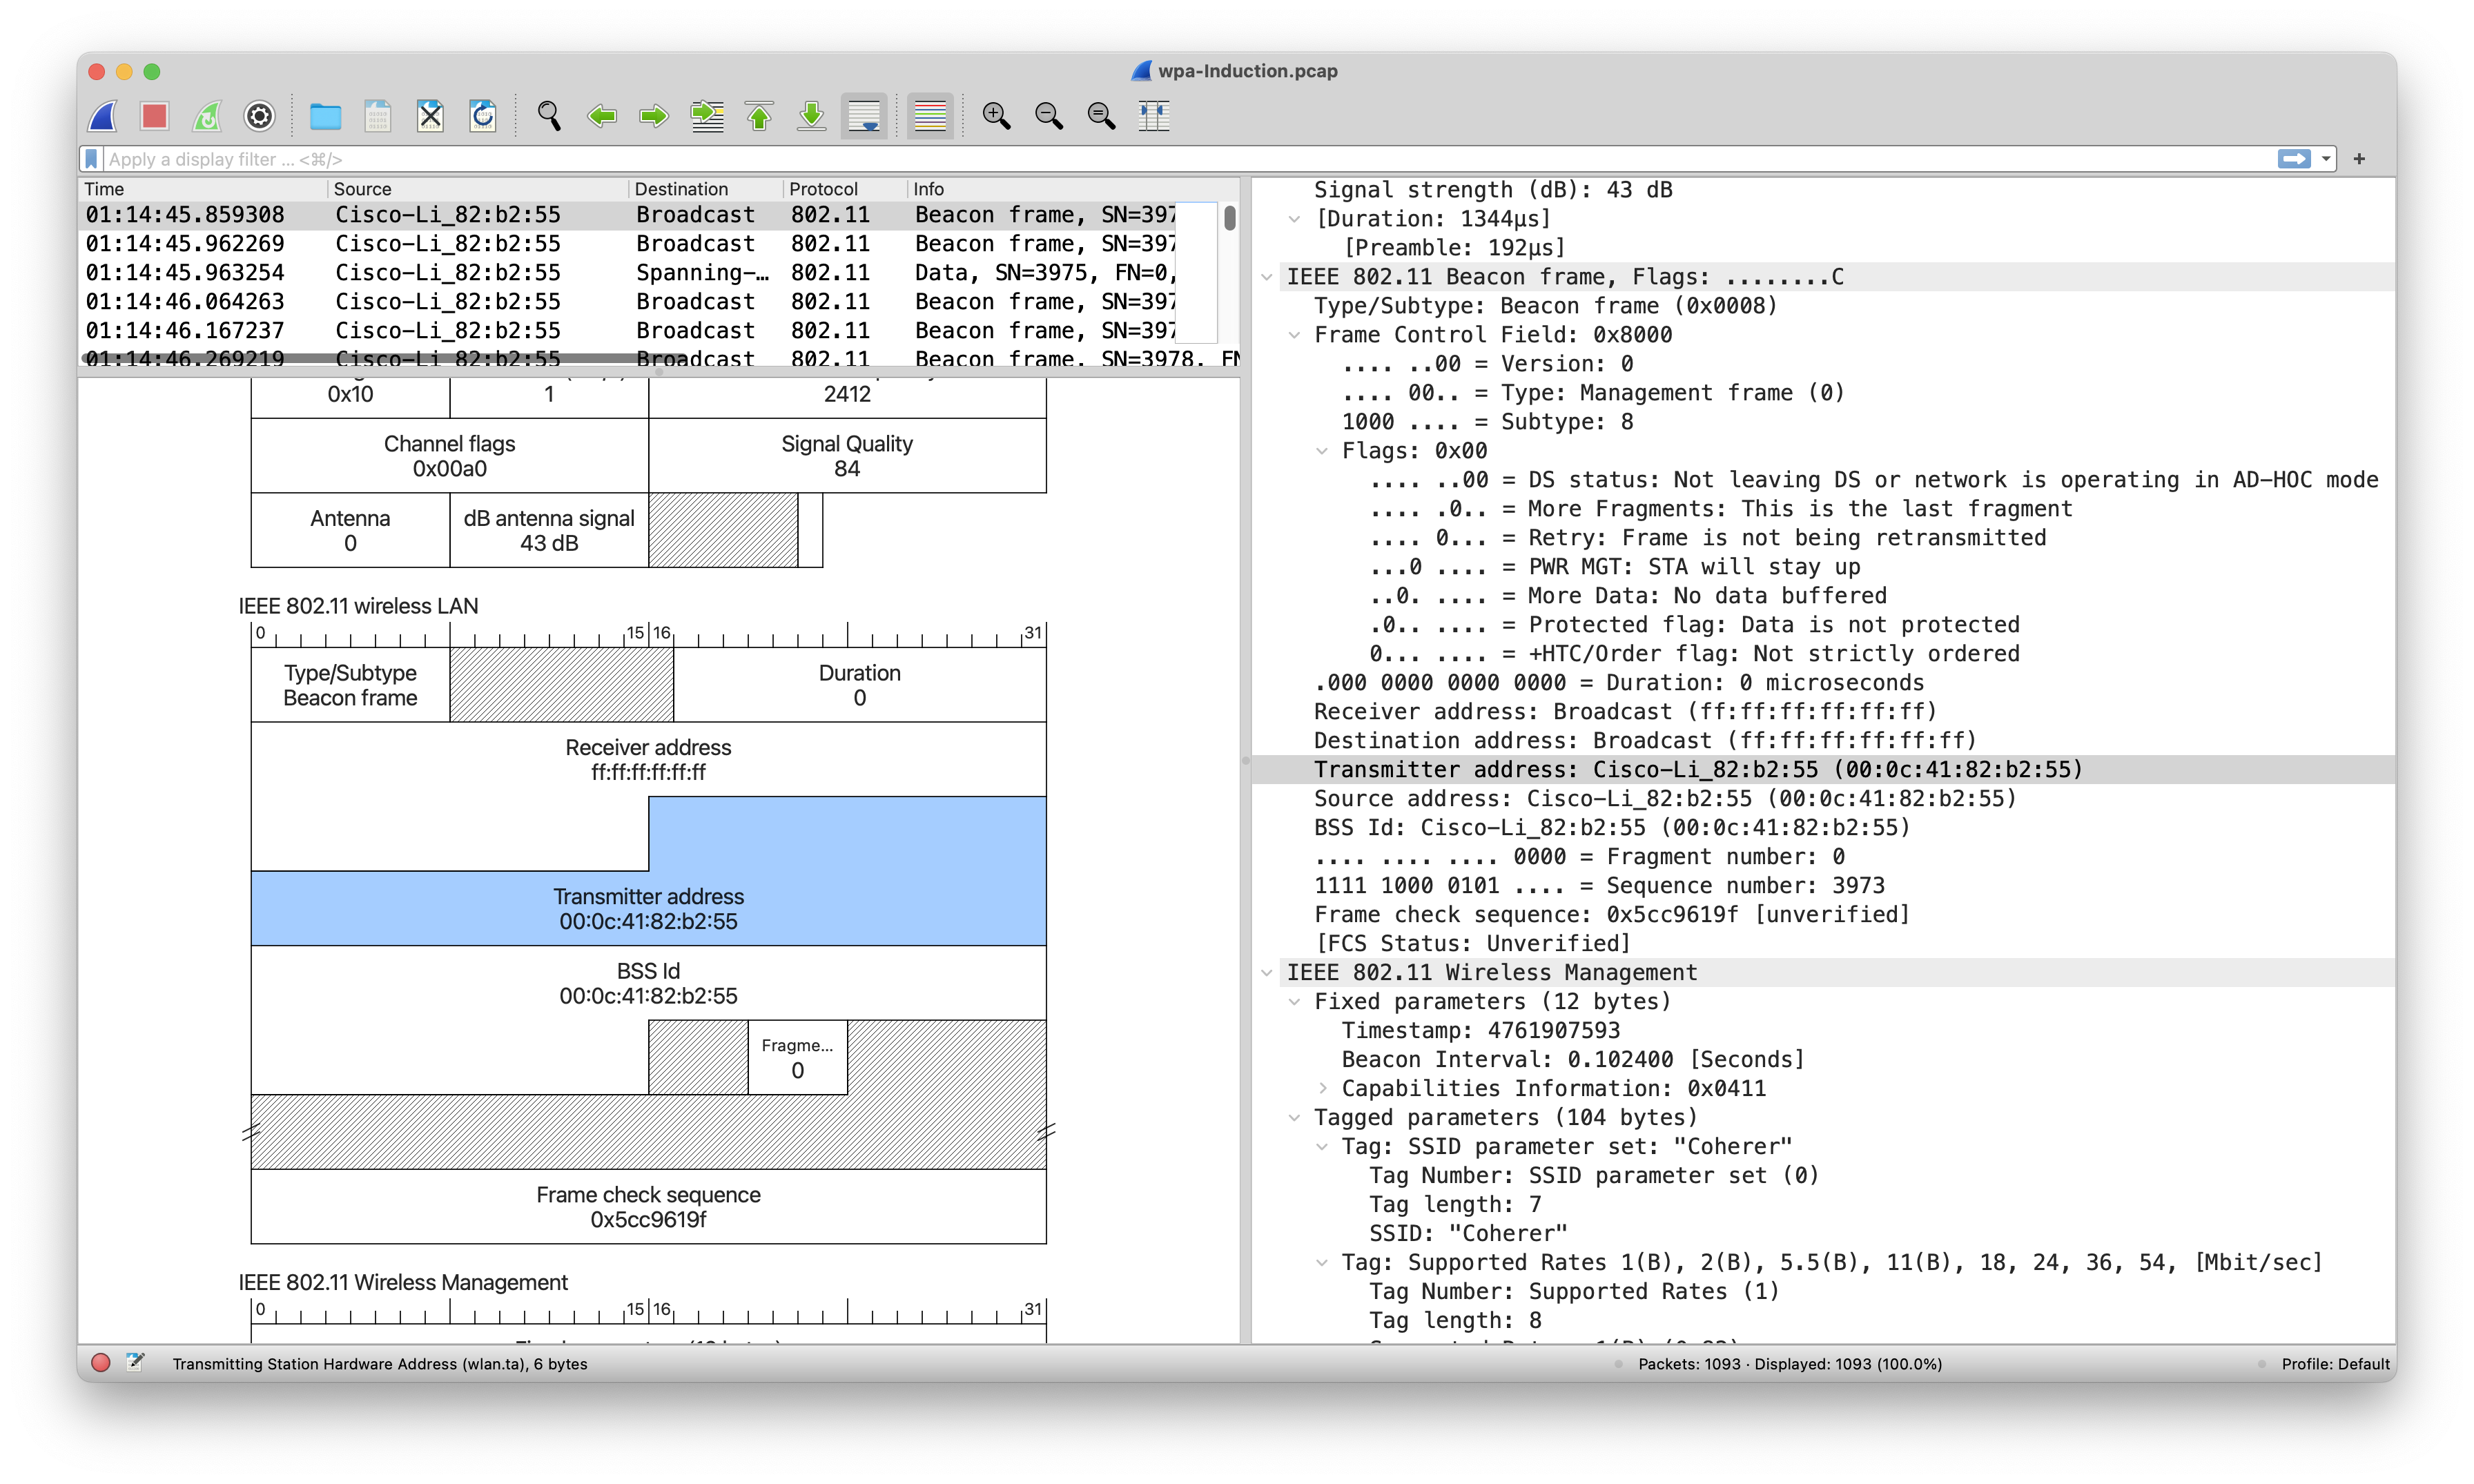
\includegraphics[width=\textwidth]{subfiles/images/PART2_Beacon_Frame.png}
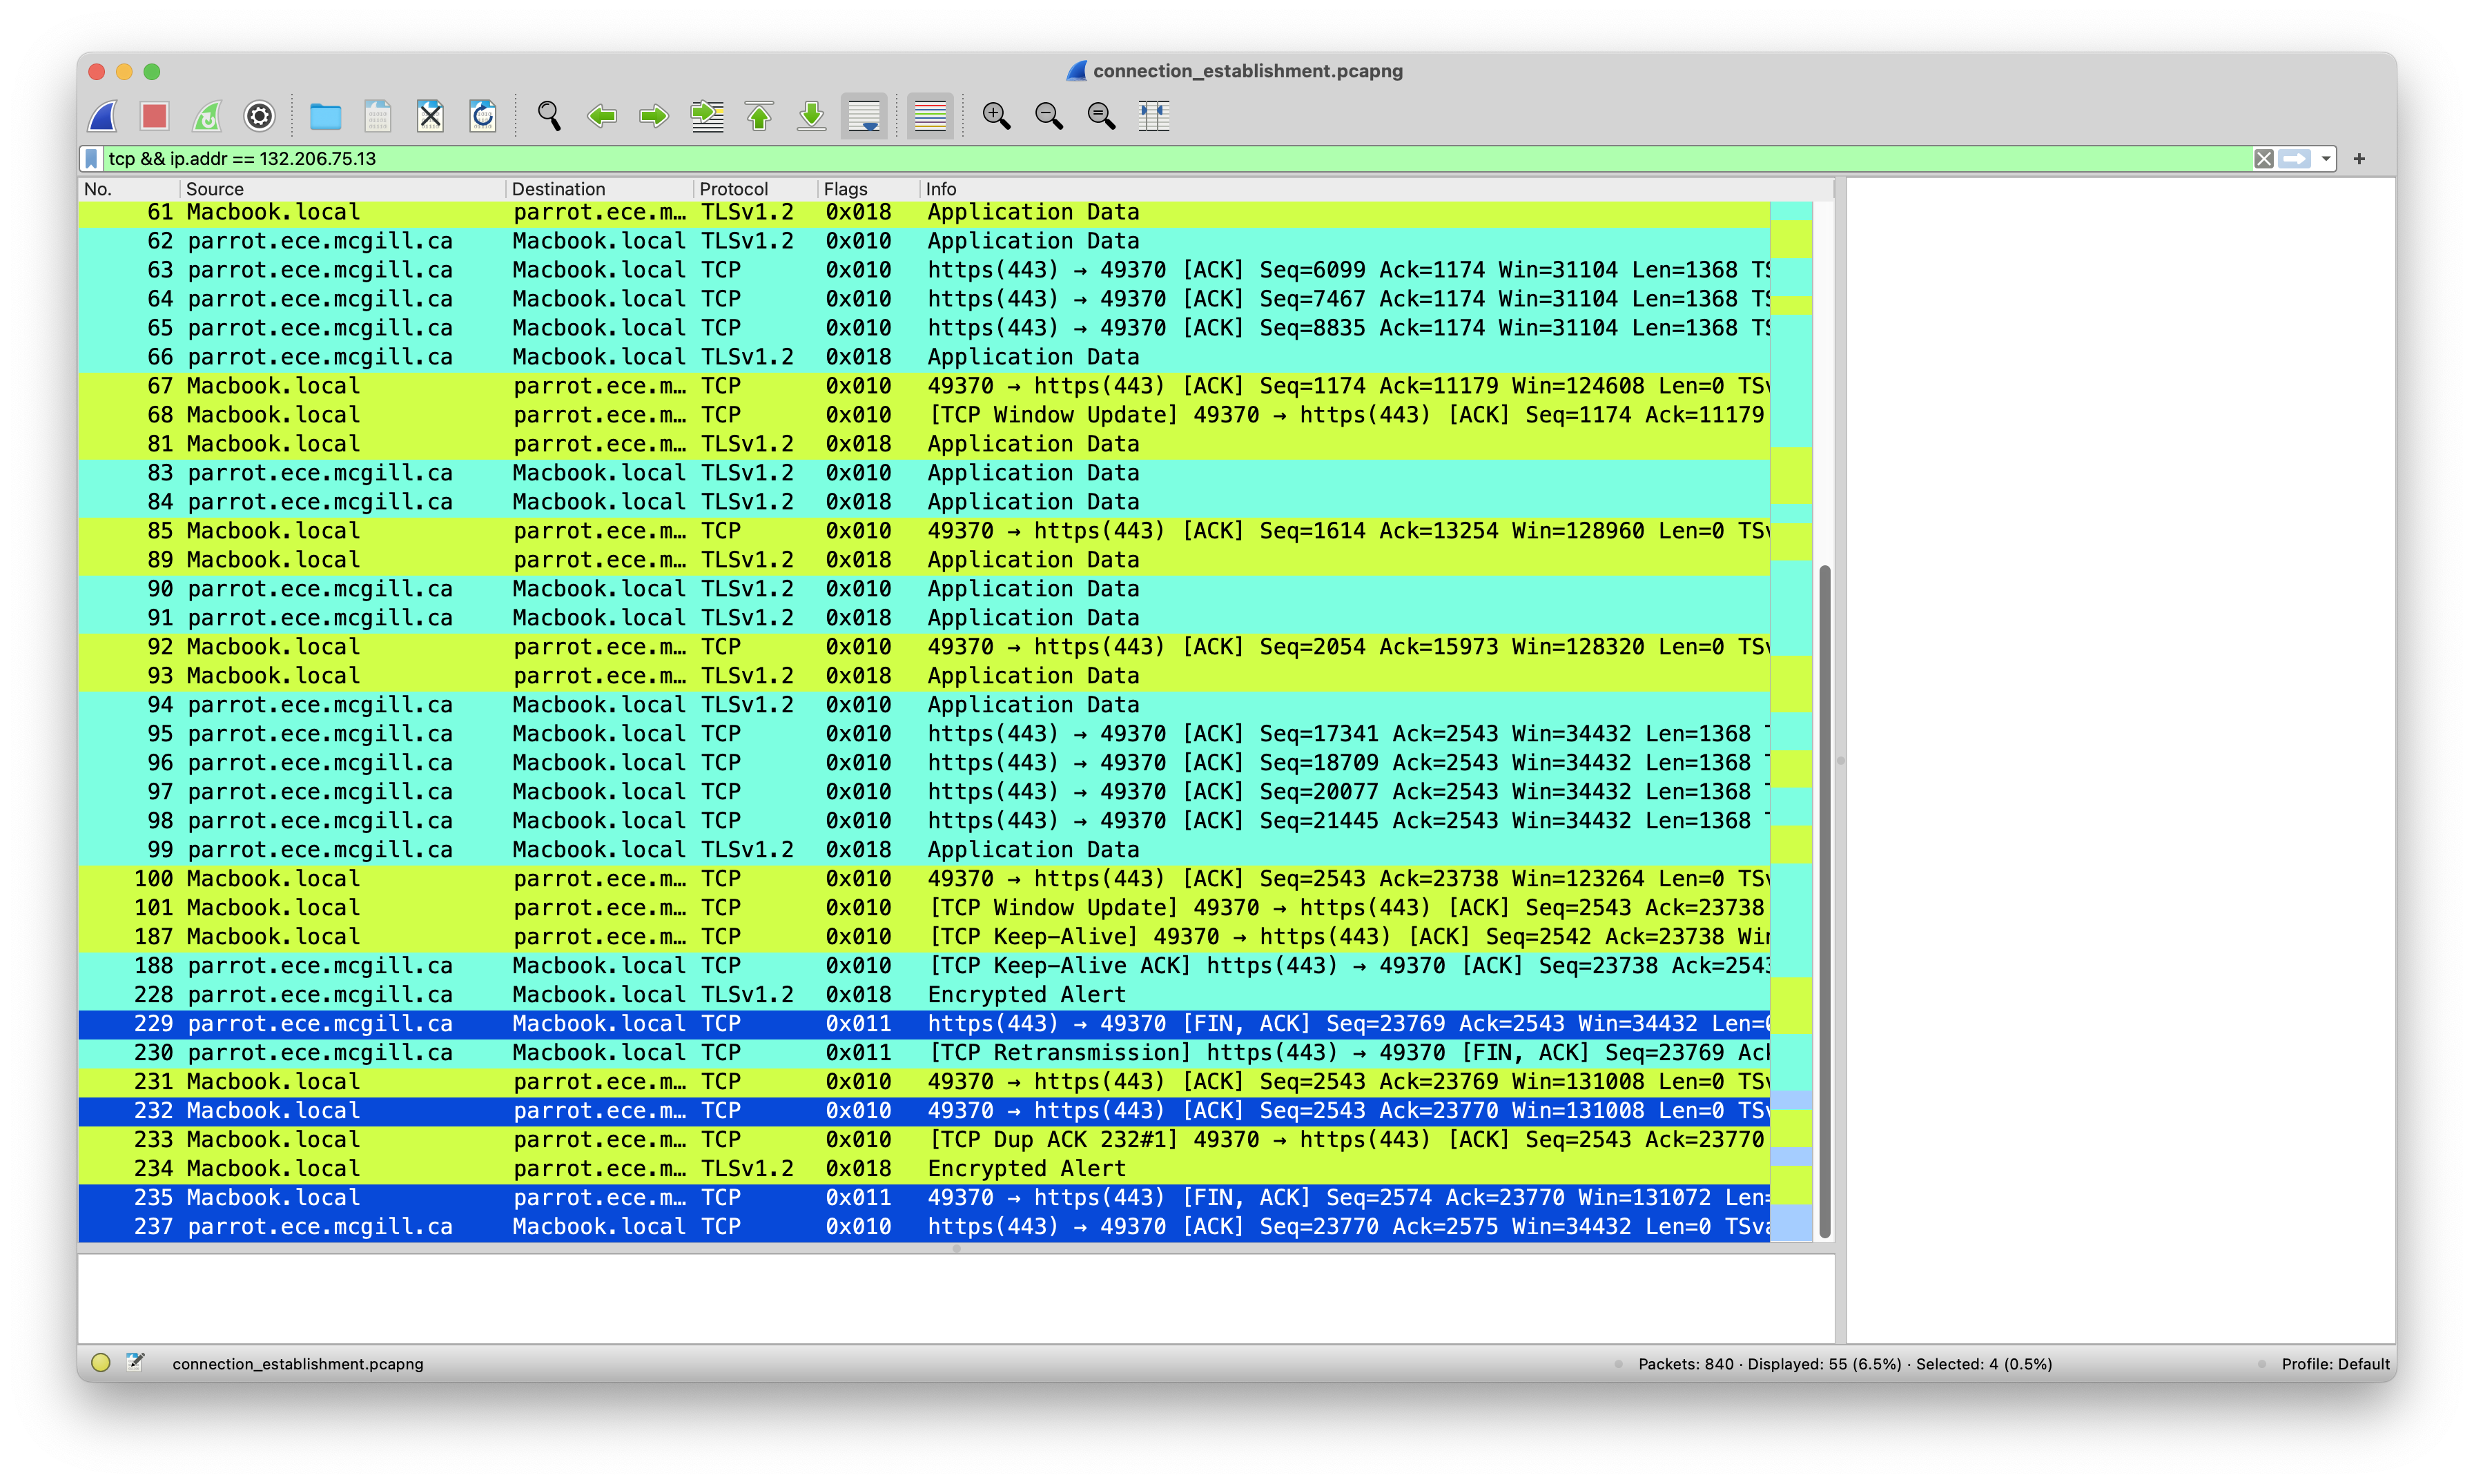
\includegraphics[width=\textwidth]{subfiles/images/CONNECTION_TERMINATION_Q16.png}
\end{proof}

\end{document}